\chapter{РЕЗУЛЬТАТЫ И ОБСУЖДЕНИЕ}

\section{Результаты физических sanity checks}
\todo{Свести результаты шага 07: energy convention, scaling, Bessel check, diagnostic-only status of $dE_2$.}

\section{Результаты physics-informed Ridge baseline}
\todo{Описать результаты Milestone 06c: Ridge как основной интерпретируемый baseline.}
\todo{Добавить таблицы MAE/RMSE после финальной подготовки текста.}

\section{Сравнение Ridge и tiny MLP}
\todo{MLP+physics succeeds in 10/16 cells overall.}
\todo{LOAO: 3/8.}
\todo{LOARO: 7/8.}
\todo{Criterion not met.}
\todo{Ridge remains preferred.}
\todo{LOAO failure concentrated in $dE_1$: all four n-classes have negative improvement for $dE_1$ under LOAO.}
\todo{For $E_0$ under LOAO, MLP improves in 3/4 n-classes.}
\todo{Conclusion: tiny MLP can add weak nonlinear corrections in some cases but does not robustly improve generalization to unseen size values for $dE_1$.}

\begin{figure}[htbp]
  \centering
  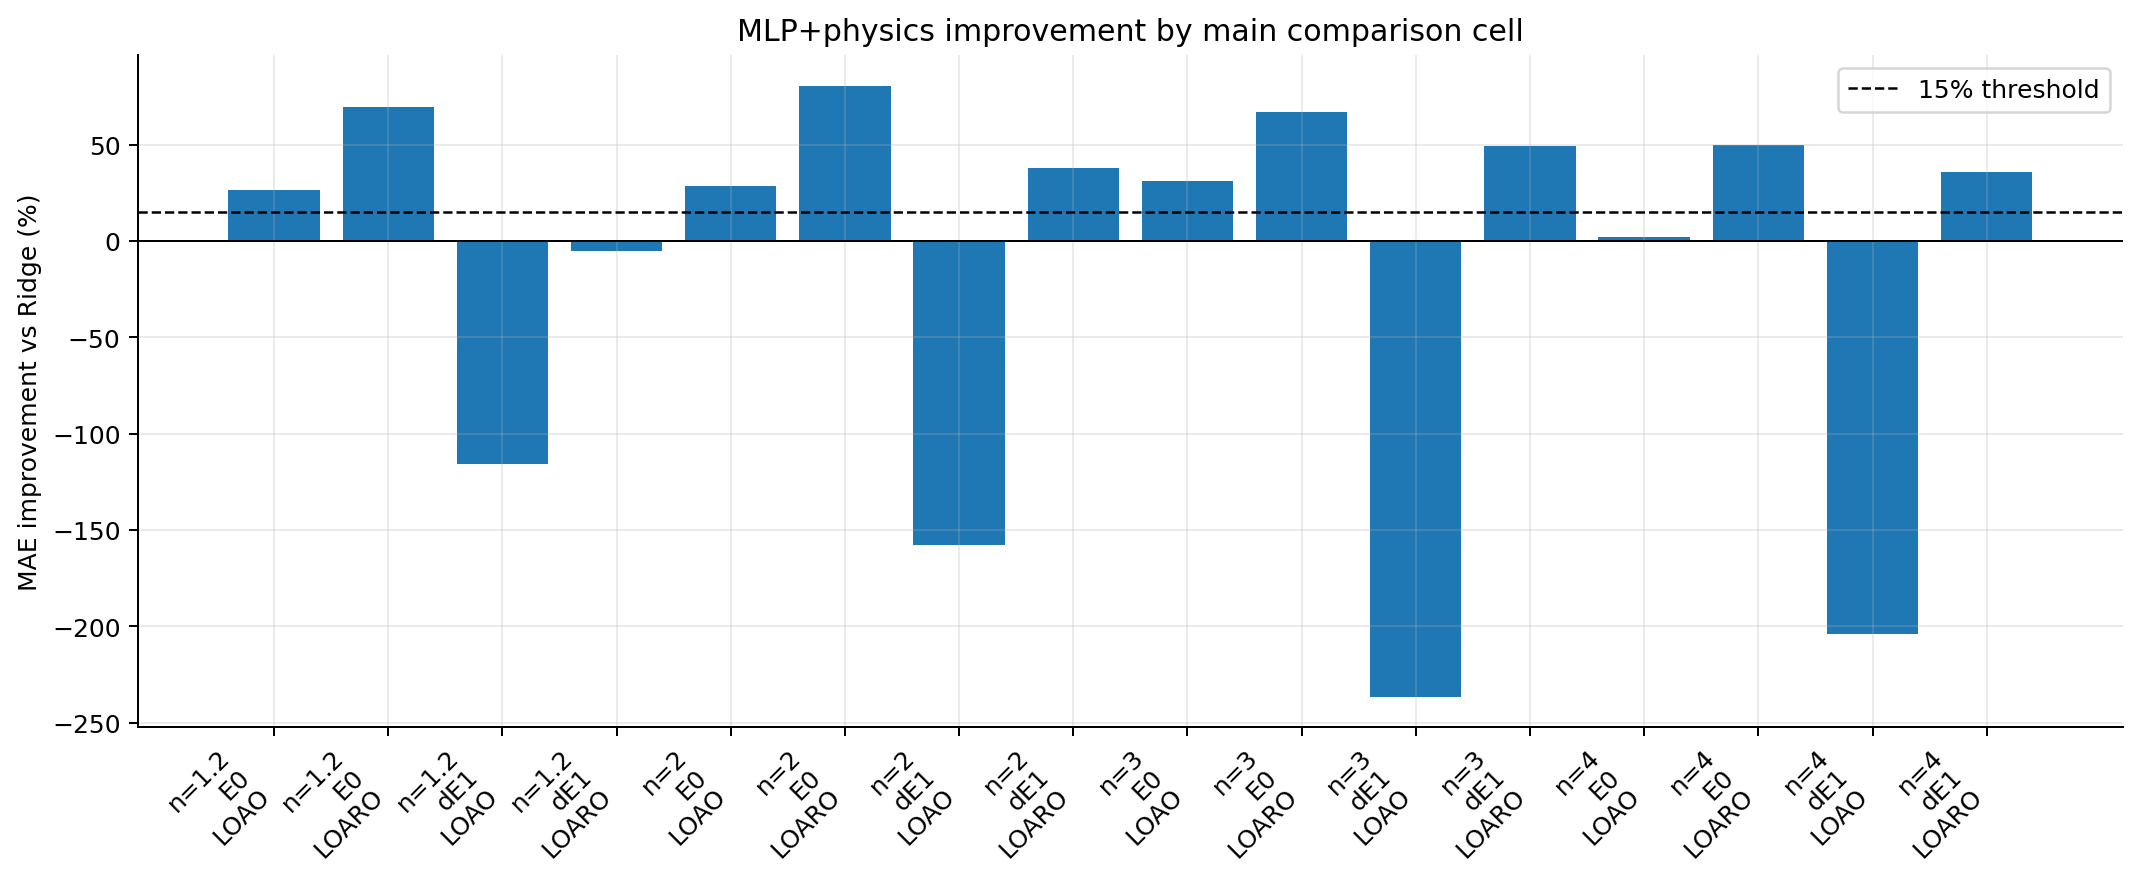
\includegraphics[width=0.85\textwidth]{../reports/assets/mlp_ablation_improvement_by_cell.png}
  \caption{TODO: Улучшение tiny MLP относительно Ridge по предрегистрационным ячейкам.}
\end{figure}

\begin{figure}[htbp]
  \centering
  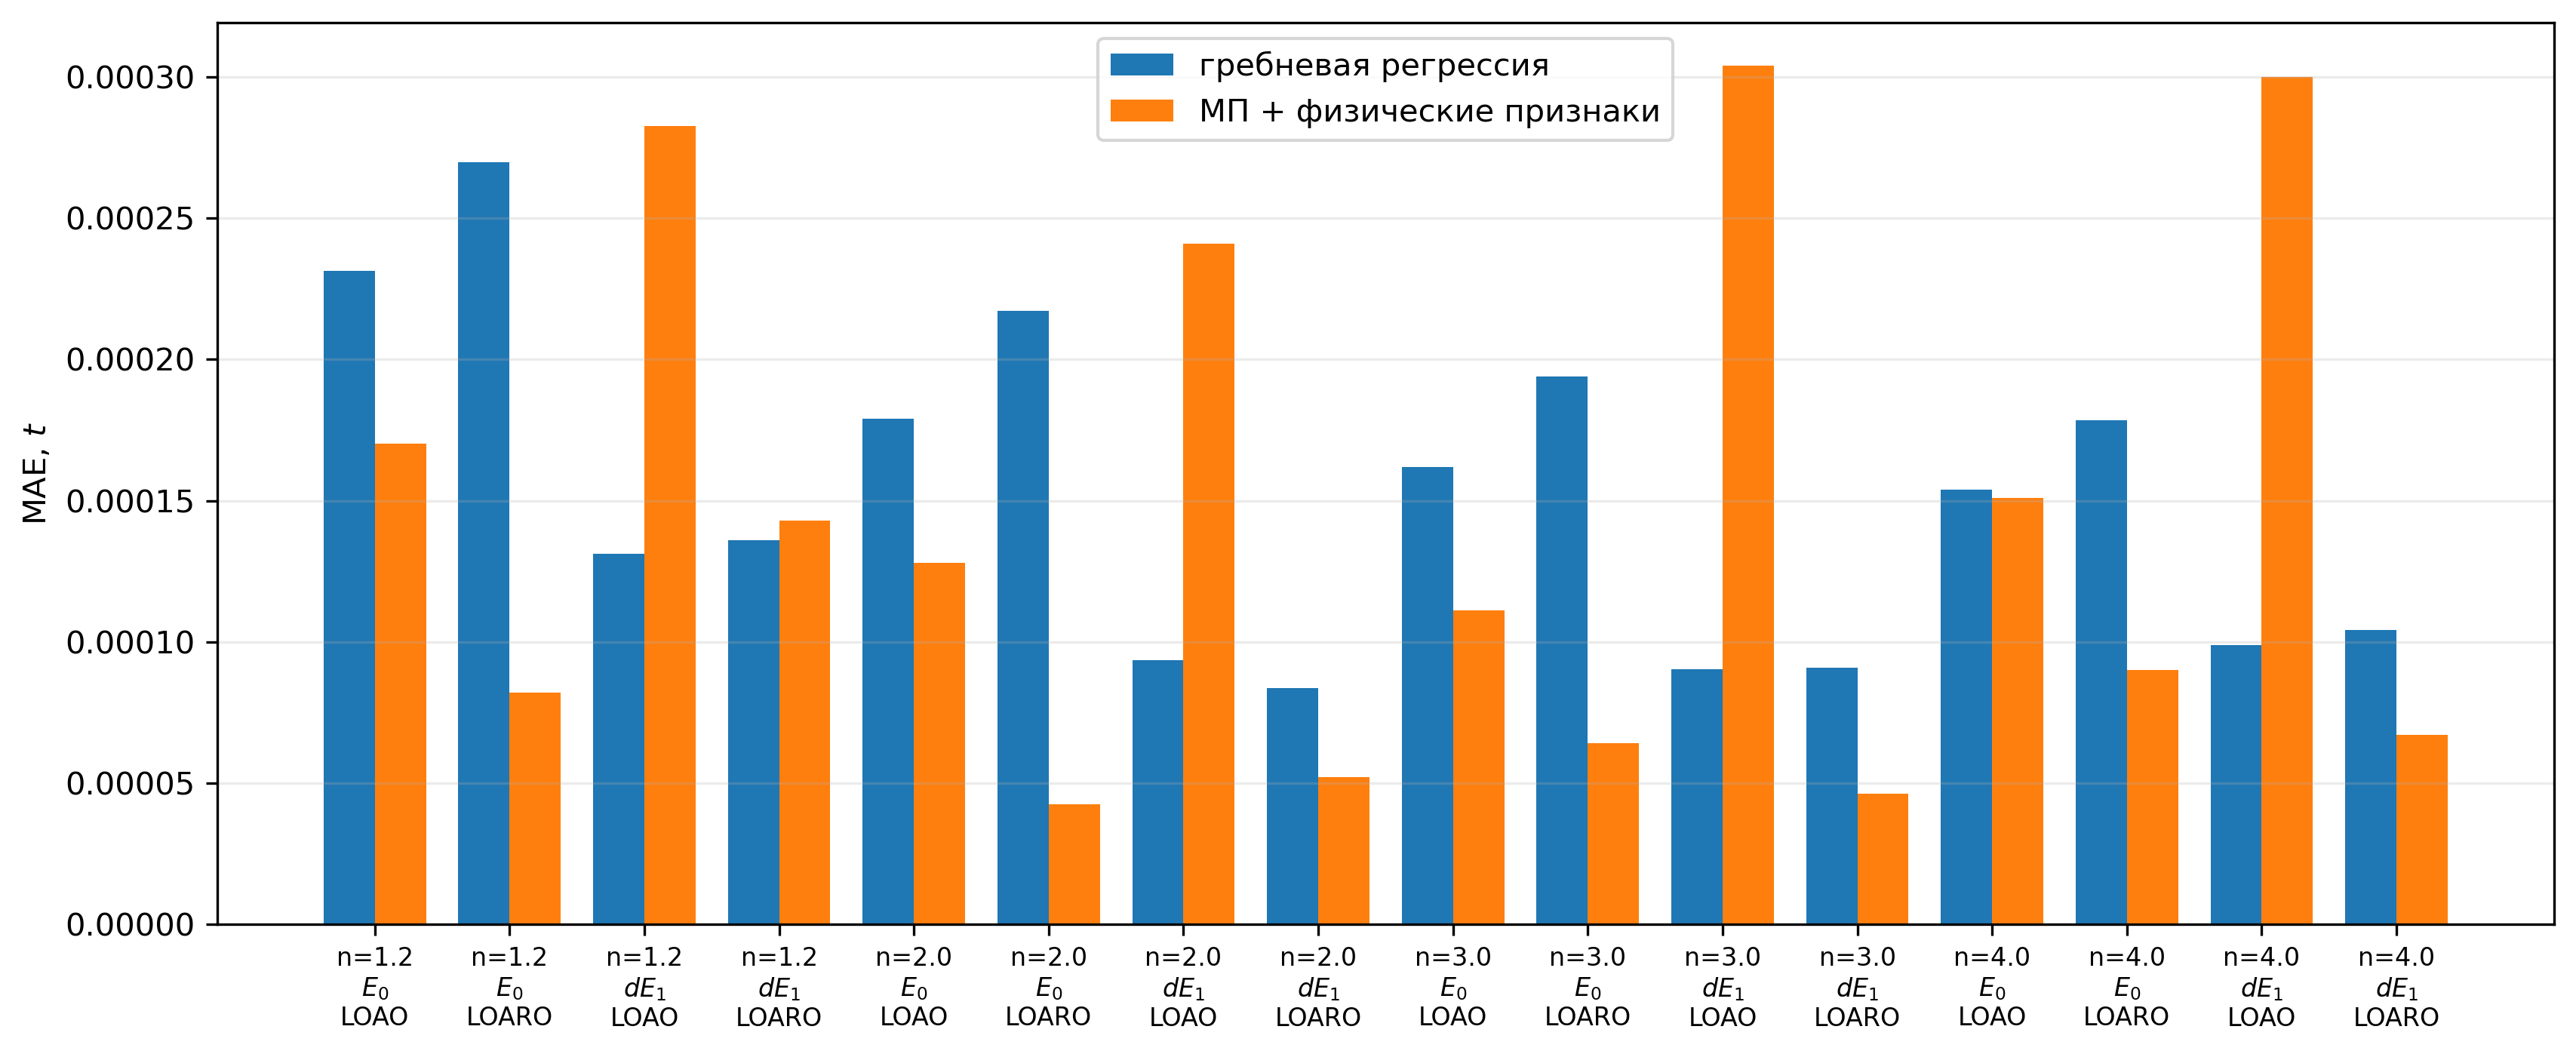
\includegraphics[width=0.85\textwidth]{../reports/assets/mlp_ablation_ridge_vs_mlp_physics_mae.png}
  \caption{TODO: Сравнение MAE Ridge и MLP+physics.}
\end{figure}

\begin{figure}[htbp]
  \centering
  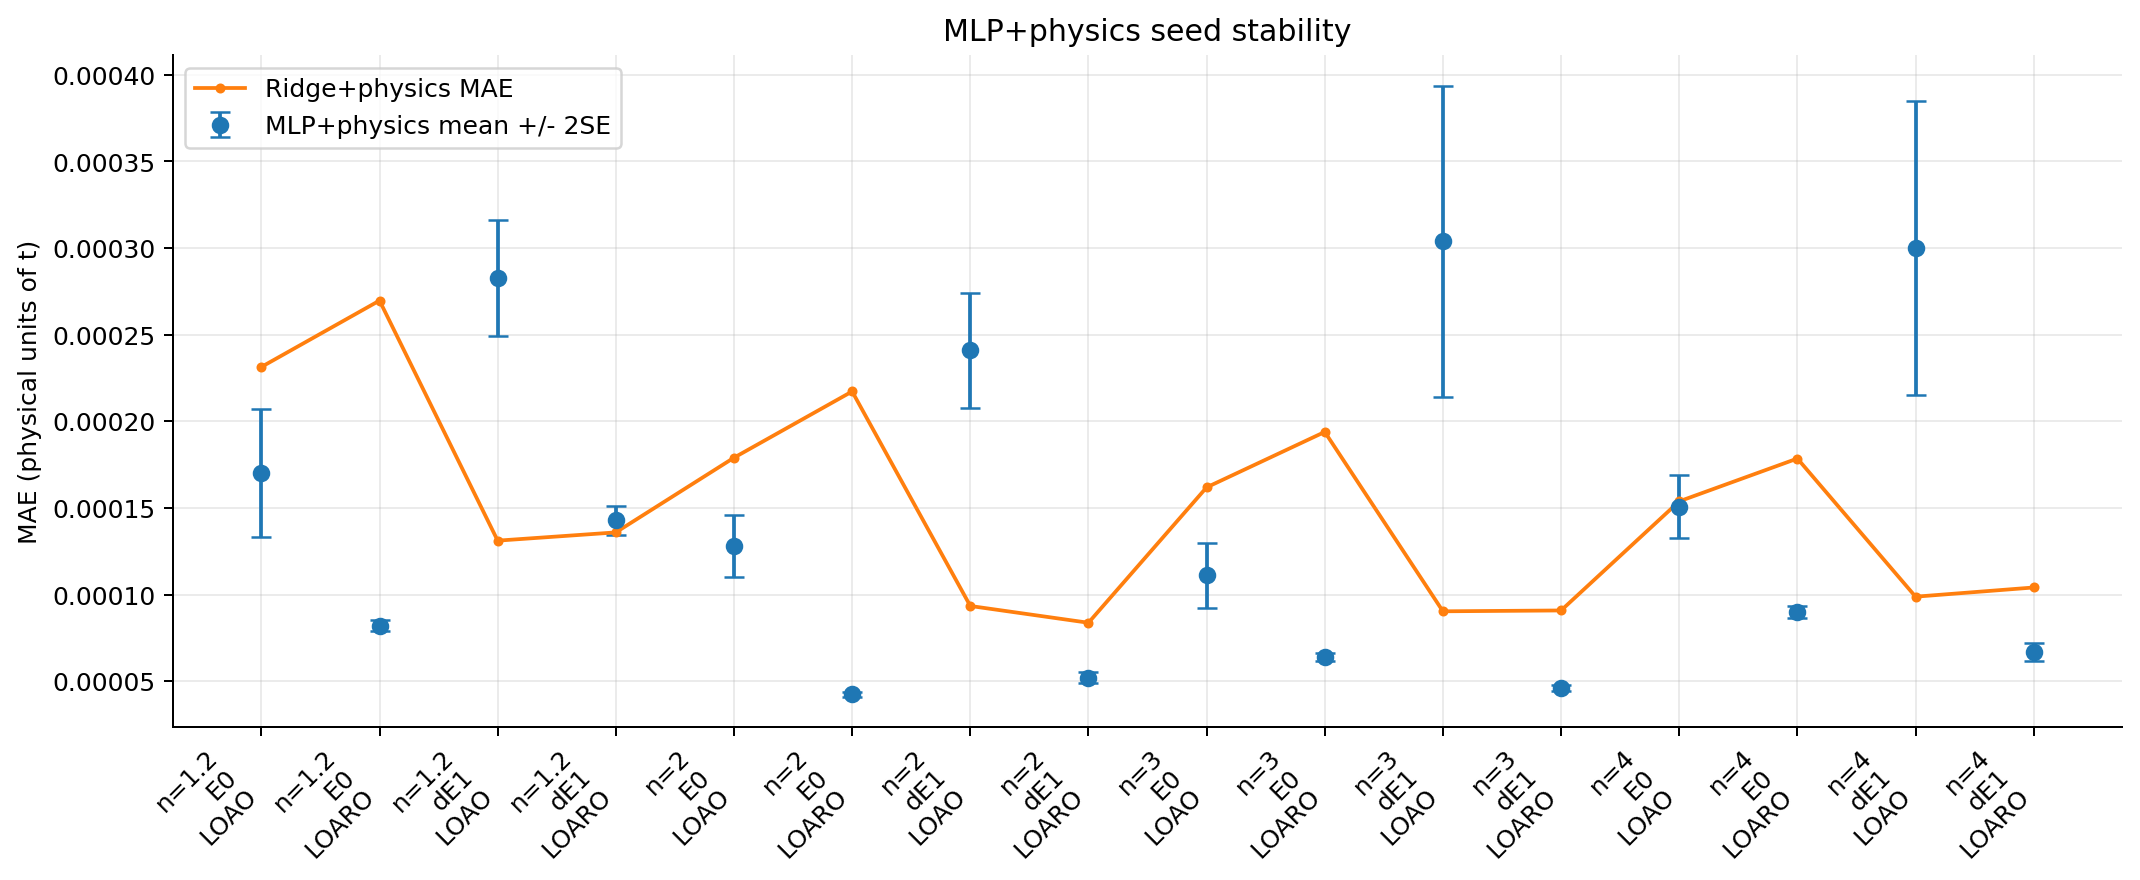
\includegraphics[width=0.85\textwidth]{../reports/assets/mlp_ablation_seed_stability.png}
  \caption{TODO: Устойчивость MLP+physics по random seeds.}
\end{figure}

\begin{figure}[htbp]
  \centering
  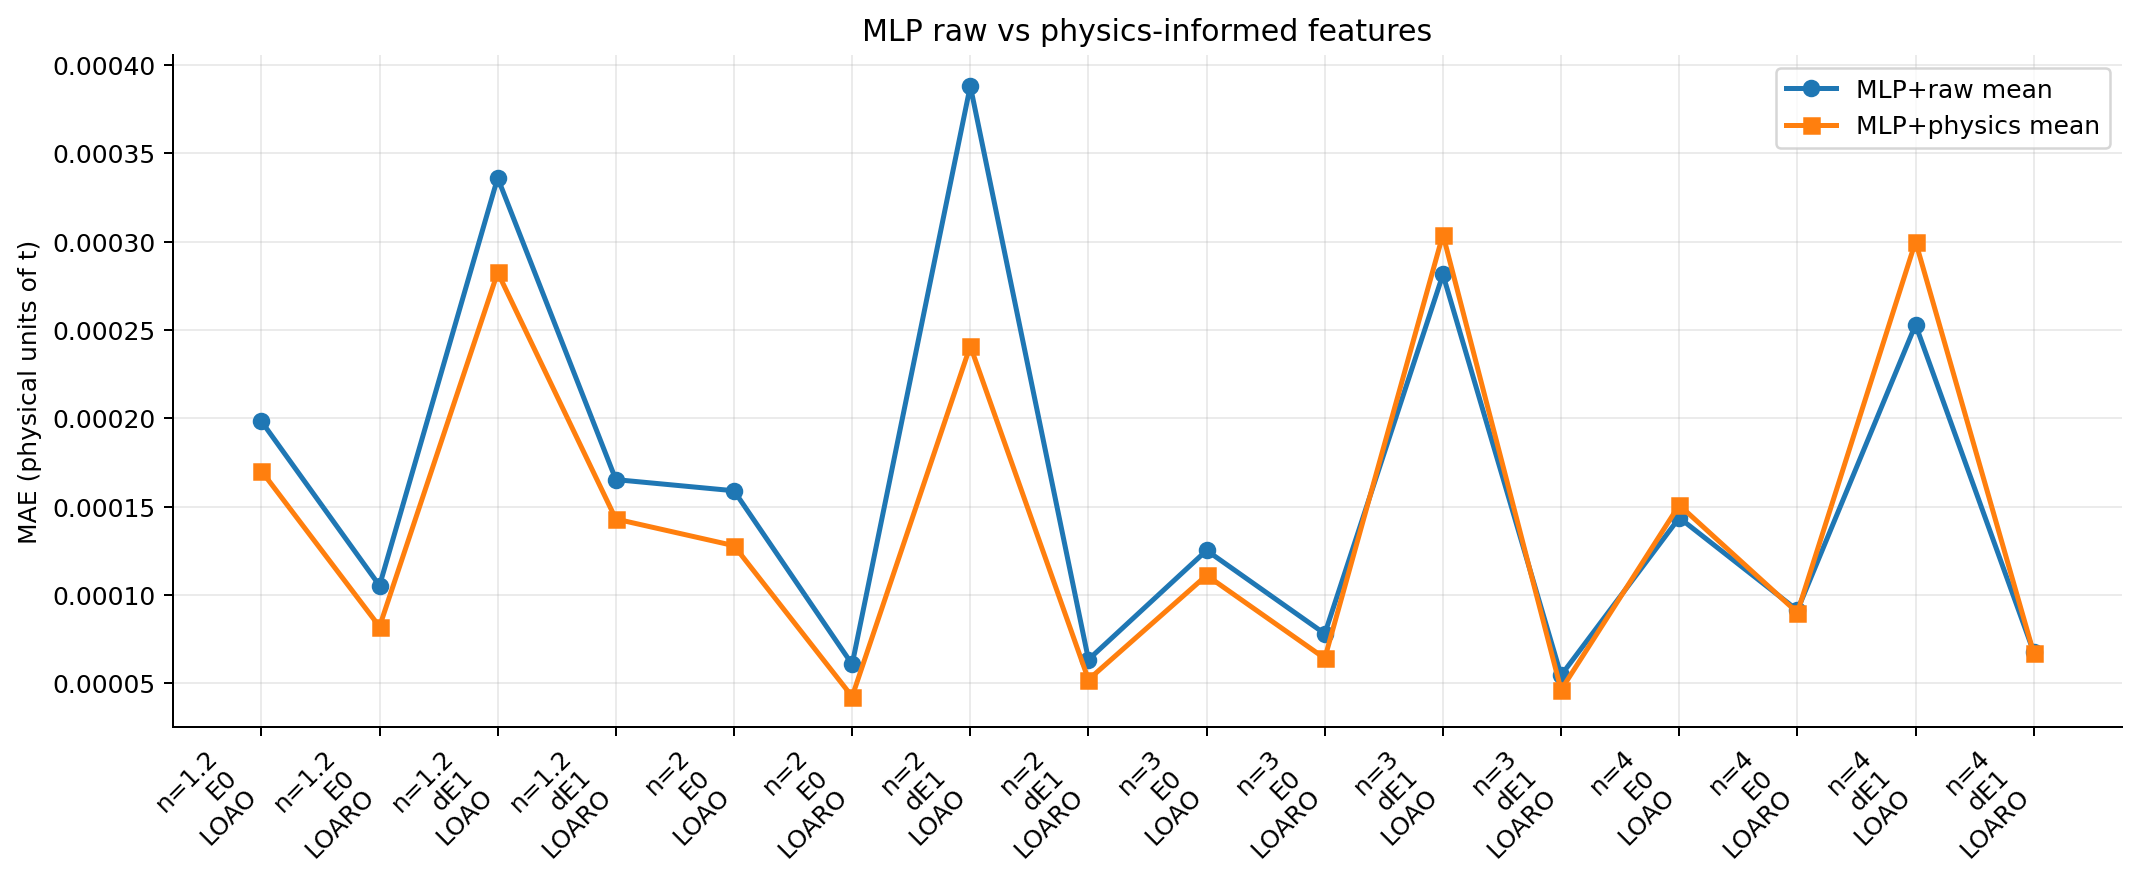
\includegraphics[width=0.85\textwidth]{../reports/assets/mlp_raw_vs_physics_features.png}
  \caption{TODO: Сравнение raw и physics-informed признаков для MLP.}
\end{figure}

\section{Анализ остатков Ridge}
\todo{Primary residual hypothesis not supported.}
\todo{Discretization dominated smooth macro-parameters in 3/4 n-classes.}
\todo{Meaningful discretization support only in 1/4 n-classes.}
\todo{Meaningful case: $n=1.2$, \texttt{imbalance\_ratio}, $\rho \approx 0.416$, $p \approx 0.013$.}
\todo{For $n \geq 2$, selected simple edge-discretization diagnostics do not systematically explain the remaining Ridge residuals.}
\todo{Mention that \texttt{imbalance\_ratio} and \texttt{abs\_delta\_N\_over\_N} are identical aliases if this is reflected in final step-09 cleanup.}

\begin{figure}[htbp]
  \centering
  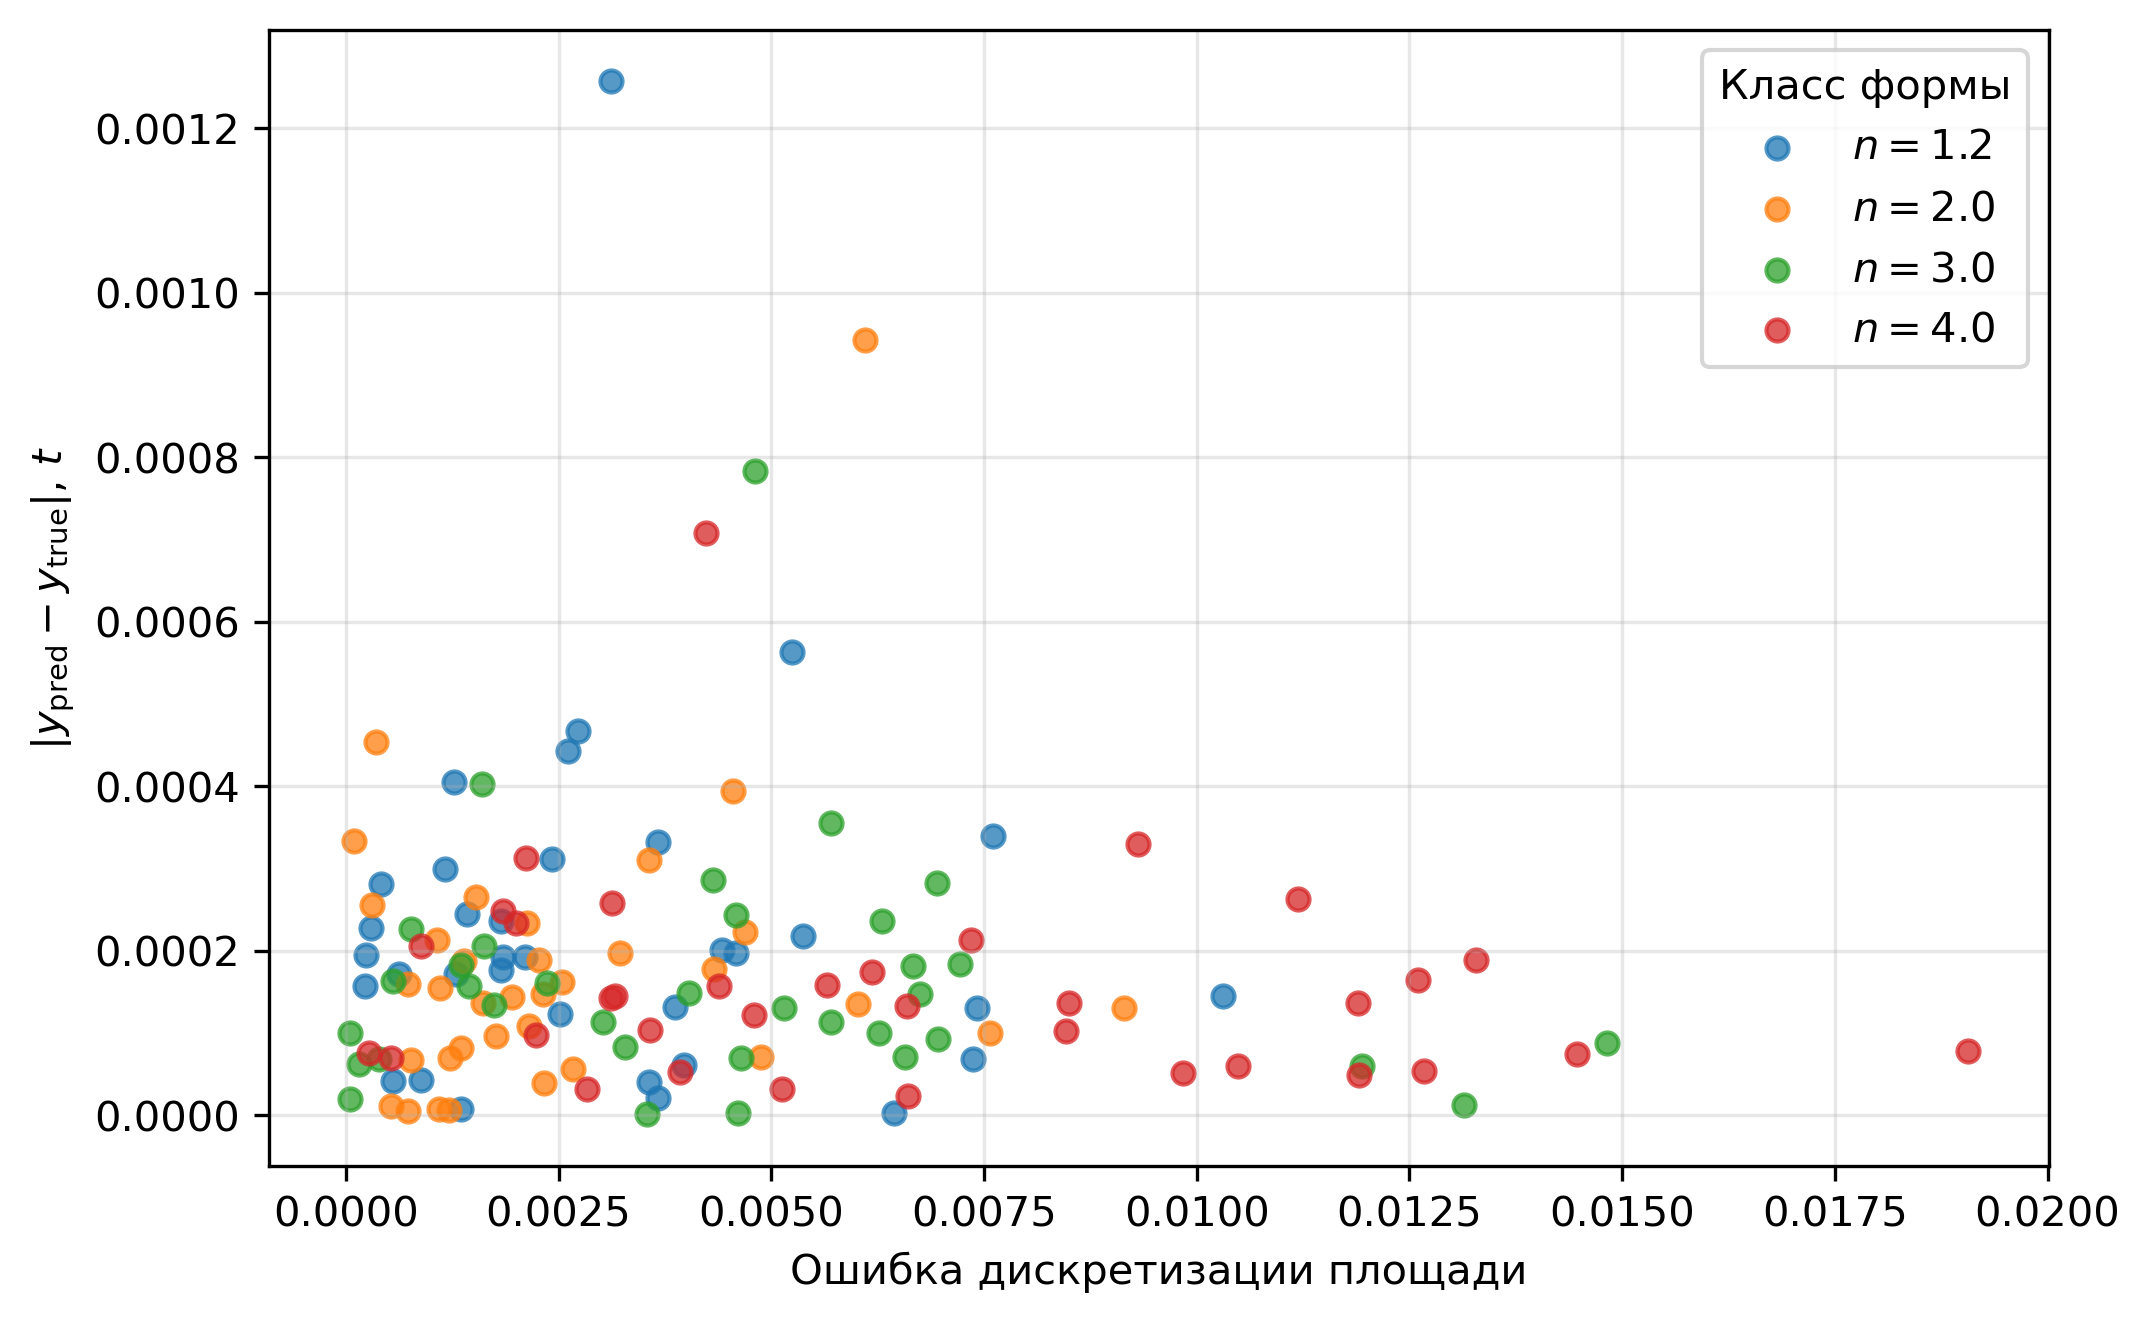
\includegraphics[width=0.85\textwidth]{../reports/assets/ridge_e0_loao_abs_residual_vs_edge_error.png}
  \caption{TODO: Остатки Ridge и ошибка дискретизации площади для E0/LOAO.}
\end{figure}

\begin{figure}[htbp]
  \centering
  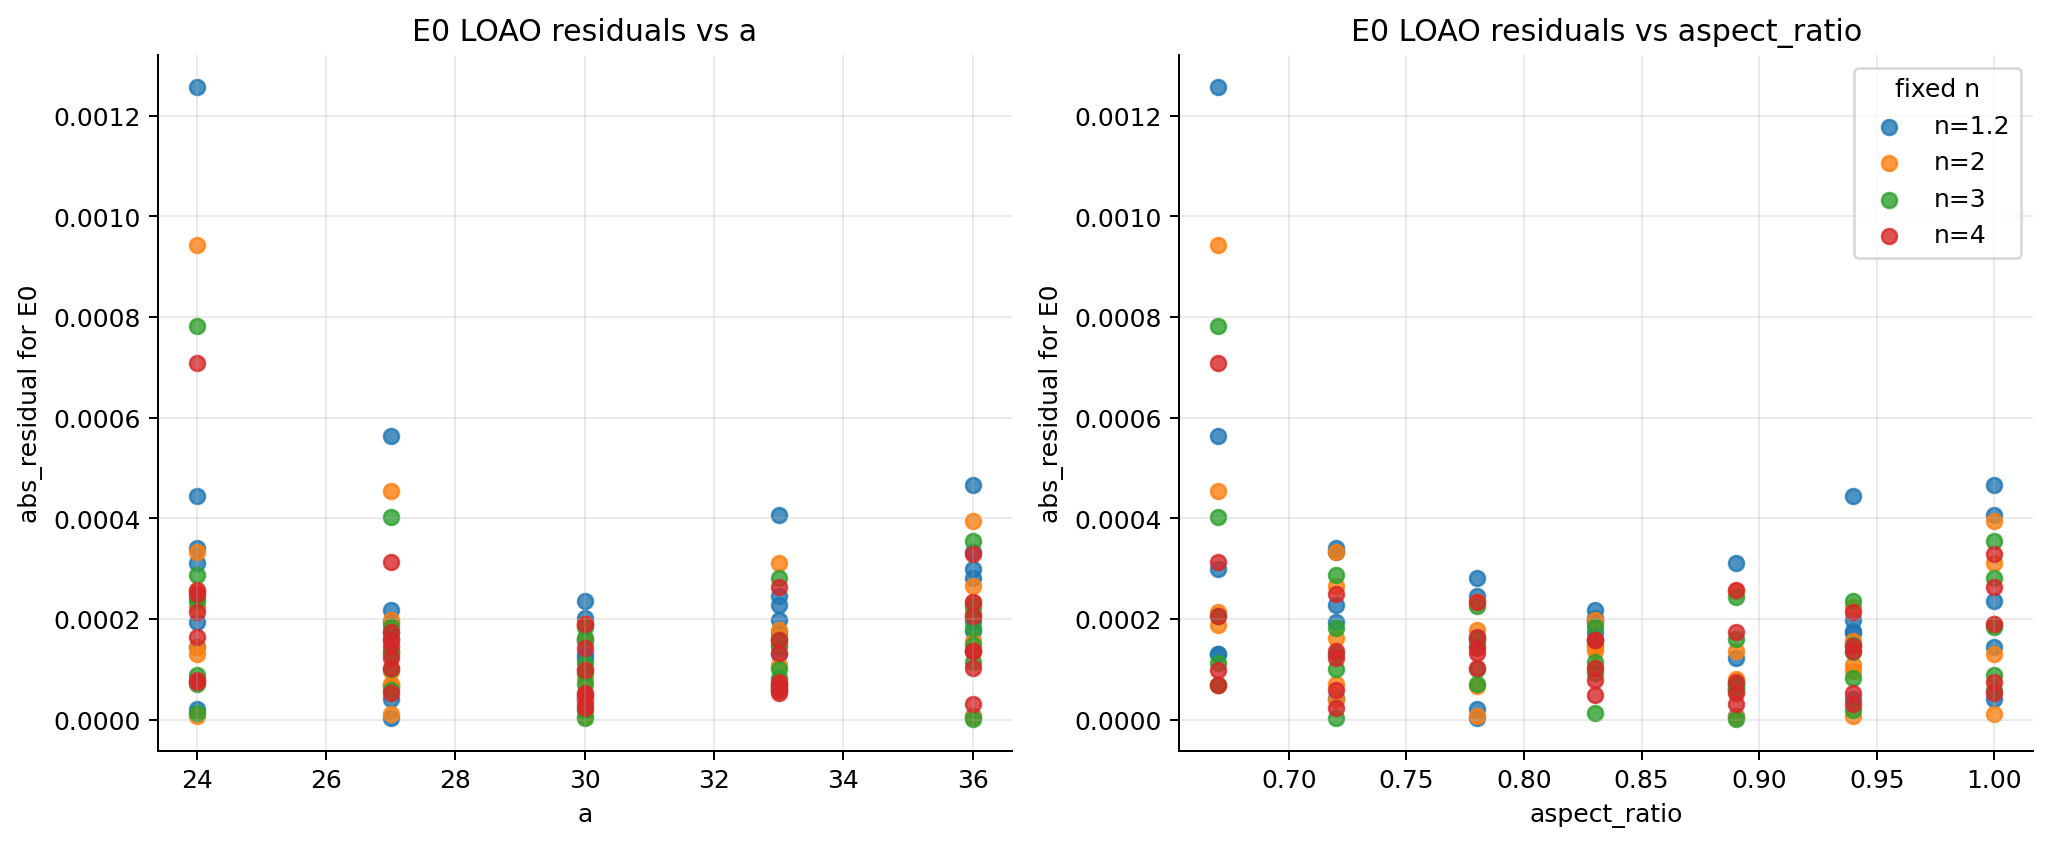
\includegraphics[width=0.85\textwidth]{../reports/assets/ridge_e0_loao_abs_residual_vs_macro_params.png}
  \caption{TODO: Остатки Ridge и гладкие макропараметры для E0/LOAO.}
\end{figure}

\begin{figure}[htbp]
  \centering
  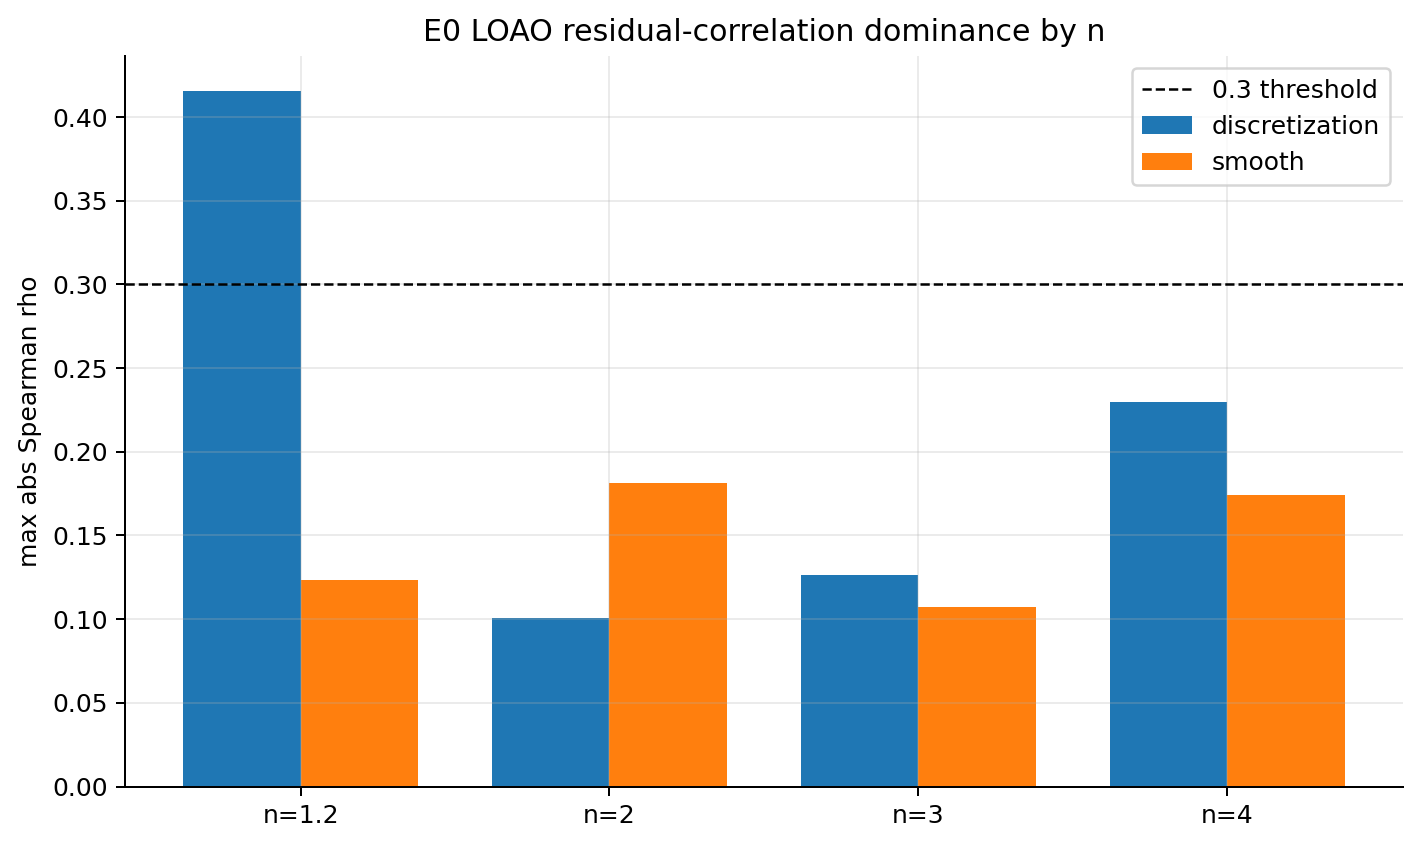
\includegraphics[width=0.85\textwidth]{../reports/assets/ridge_residual_dominance_by_n.png}
  \caption{TODO: Сравнение максимальных Spearman-корреляций по классам $n$.}
\end{figure}

\begin{figure}[htbp]
  \centering
  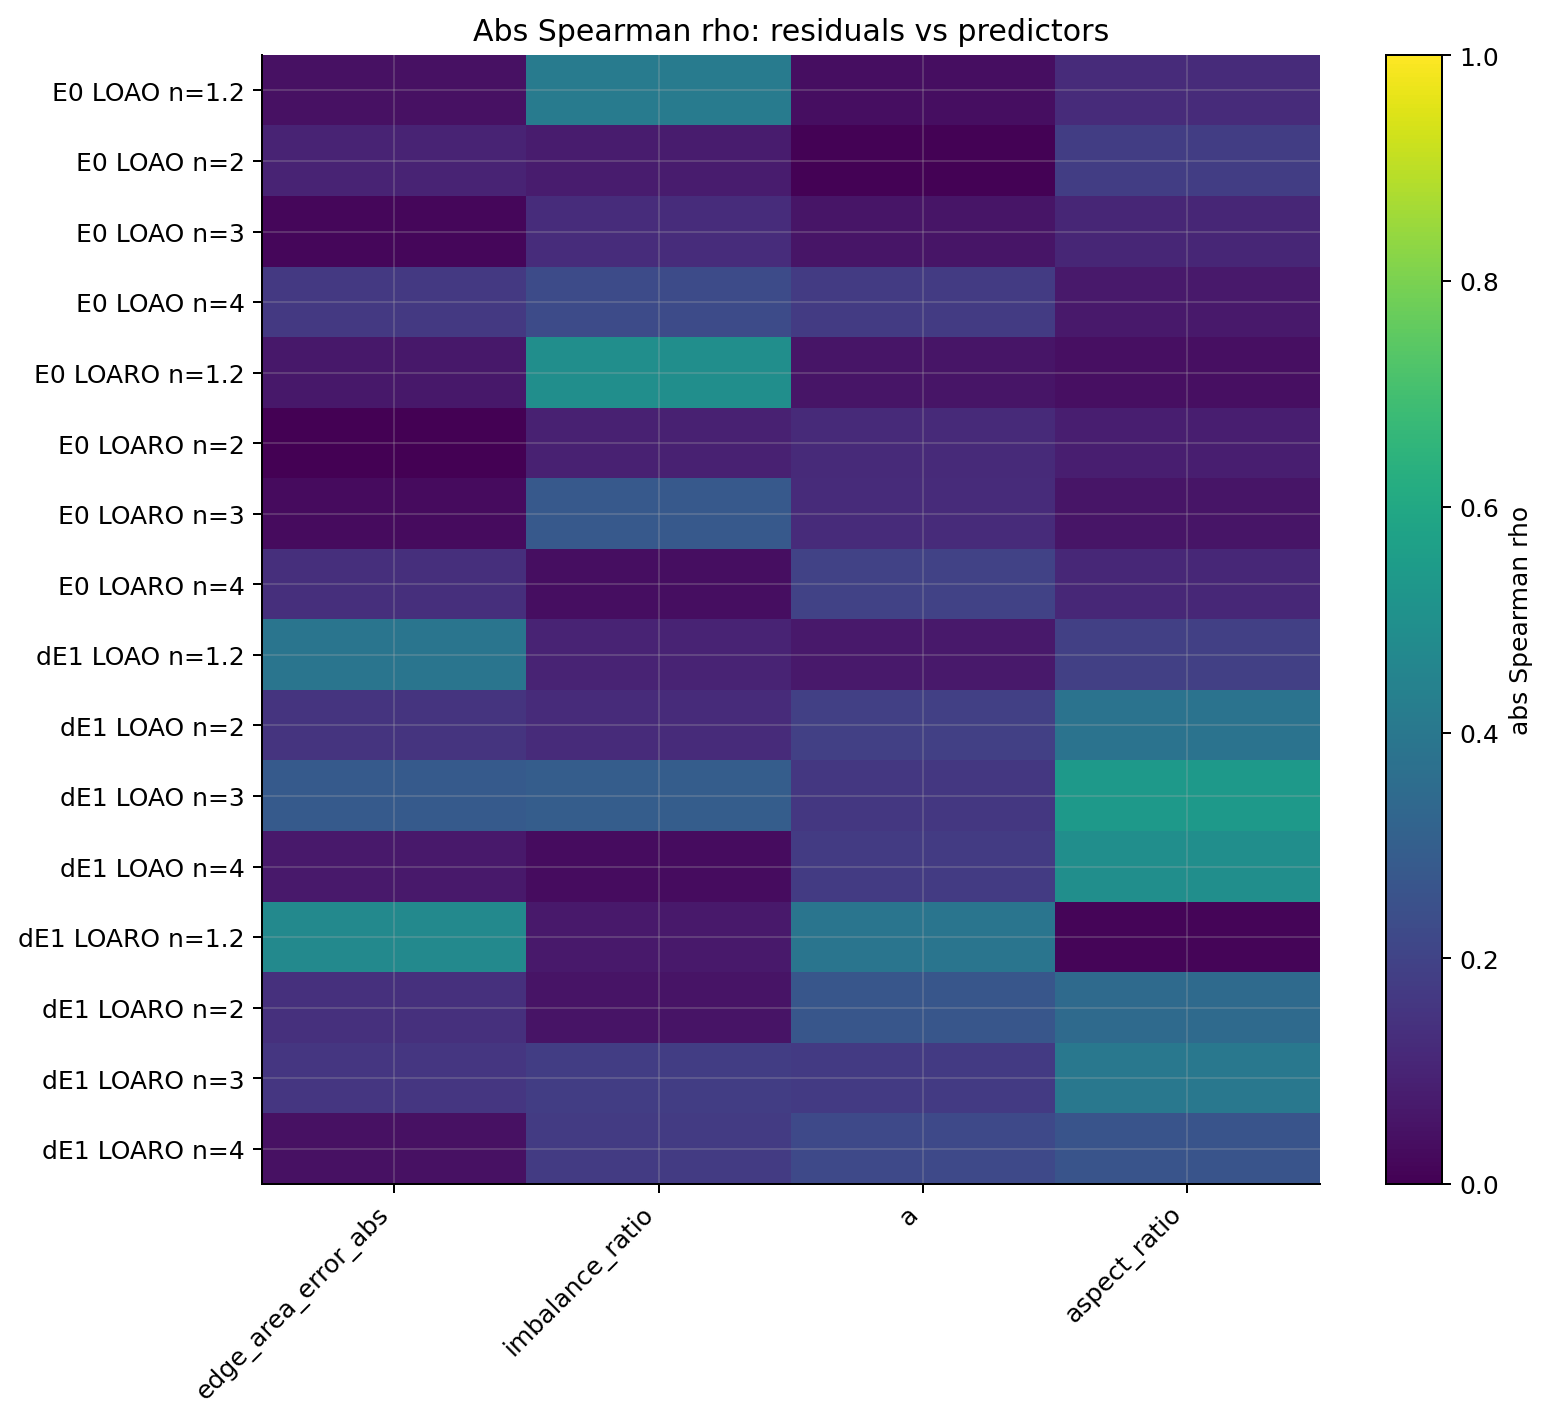
\includegraphics[width=0.85\textwidth]{../reports/assets/ridge_residual_correlation_heatmap.png}
  \caption{TODO: Карта корреляций остатков с диагностическими переменными.}
\end{figure}

\section{Проверяемый сценарий surrogate-assisted inverse screening}
\todo{This section is optional until step 10 is completed.}
\todo{Use Ridge only as a fast candidate filter.}
\todo{Validate all selected candidates by direct Kwant calculation.}
\todo{Do not present the surrogate as a substitute for direct Kwant validation.}
\todo{Stay inside the verified design window.}

\section{Ограничения применимости и связь с задачами нанодизайна}
\todo{Model is square-lattice TB, not material-specific DFT.}
\todo{No claim for arbitrary $n$.}
\todo{No claim for arbitrary shapes.}
\todo{No claim that MLP is unnecessary in all contexts.}
\todo{No claim that residuals are fully explained.}
\todo{Future work: DFT/OpenMX or material-specific TB calibration.}

\section{Выводы по главе 5}
\todo{Сформулировать выводы после завершения optional step 10 или явно отметить отсутствие inverse-screening результата.}

\clearpage
